\documentclass[working, oneside]{inputs/tuftebook}
%%%%%%%%%%%%%%%%%%%%
%% SUPER PREAMBLE %%
%%%%%%%%%%%%%%%%%%%%

\documentclass[a4paper]{article}
\usepackage[utf8]{inputenc}
\usepackage[T1]{fontenc} % Fonts and stuff
\usepackage{amsmath, amsfonts, mathtools, amsthm, amssymb} % math

\usepackage{fancyhdr} % Header, Footer etc.
\usepackage{adforn}

\pagestyle{fancy}
\fancyhf{}
\fancyhead[R]{Albert Lunde, John Faxe Jensen}
\fancyfoot[C]{\adforn{17}\quad\thepage\quad\adforn{45}}

\renewcommand{\headrule}{%
	\hrulefill
	 {\quad\adforn{21}\adforn{10}\adforn{49}\quad}%
	\hrulefill}
\renewcommand{\footrulewidth}{0pt}

%% Margin Control %%

\def\changemargin#1#2{\list{}{\rightmargin#2\leftmargin#1}\item[]}
\let\endchangemargin=\endlist


%%%%%%%%%%%%%%%%%%%%%%%%%%%%%%%%%%%%%%%%%%%%%%%%%%%%%%%%%%

% figure support

\usepackage{import}
\usepackage{pdfpages}
\usepackage{transparent}
\usepackage{xcolor}

\newcommand{\incfig}[2][1]{%
    \def\svgwidth{#1\columnwidth}
    \import{figures/}{#2.pdf_tex}
}

\pdfsuppresswarningpagegroup=1

%%%%%%%%%%%%%%%%%%%%%%%%%%%%%%%%%%%%%%%%%%%%%%%%%%%%%%%%%%

\usepackage{tikzsymbols} % Symbols
\usepackage{mdframed} % Boxes around theorem environments
\usepackage{thmtools}


% Exercise environment with surrounding box

\declaretheoremstyle[
    name=Exercise,
    mdframed={
  skipabove=0pt,
  skipbelow=20pt,
  innerleftmargin=10pt,
  innerrightmargin=10pt,
  innerbottommargin=7pt}
]{thmsty}
\declaretheorem[style=thmsty,numbered=no]{exercise}

% Solution environment, with coffee cup

\newenvironment{solution}
 {\renewcommand\qedsymbol{\tikzsymbolsuse{Coffeecup}}\begin{proof}[Solution]}
 {\end{proof}}

% Subexercise enviroment
%  \newenvironment{subexercise}[1]
%  {
% 	\begin{changemargin}{1.0cm}{1.0cm}
% 	\textbf{(#1)}\em
% 	}{
	% \end{changemargin}
	% } 

 \newenvironment{subexercise}[1]
 {\noindent
	 \textbf{(#1)} \quad \adforn{10} \quad \em
 }{}

% Mathematical typesetting stuff.

 \newcommand{\dd}{\mathrm{\textbf{d}}}



\usepackage{pdfpages}

\usepackage{lipsum}
\usepackage{parskip}
\usepackage{titletoc}

\usepackage{cmbright}
\usepackage{bm}
\addbibresource{bibliography.bib}

\begin{document}
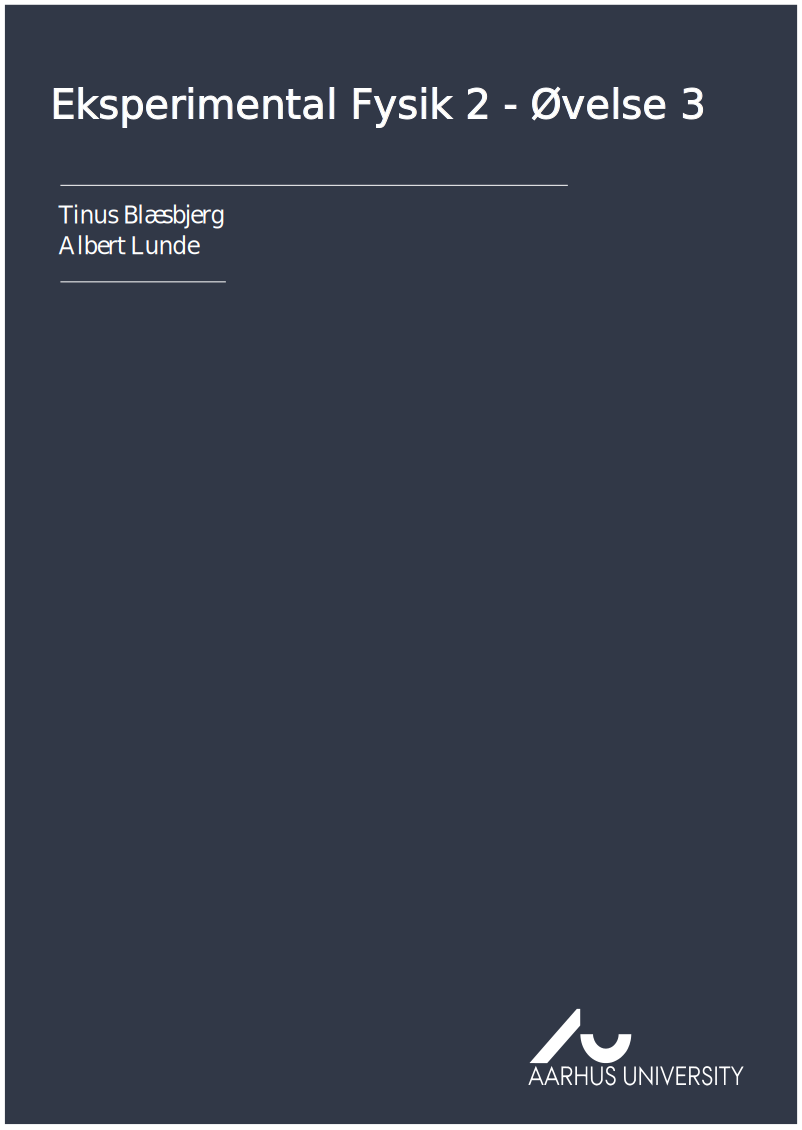
\includepdf[pages=-, fitpaper=true]{inputs/frontmatter.pdf}
\section*{Introduction}
In this experiment we construct the Mach-Zender interferometer and use this setup to examine two distinct scenarios. In the first part we look at the effects of polarizing one of the beams. In the second part we examine the interference pattern as one of the beams passes is passed through a gas with varying pressure.
\section*{Theory}
\subsection*{Waveplate and Polarization}
We shall use the following notation to describe $\bm{\hat{p}}$ and $\bm{\hat{s}}$-polarized waves, where these vectors describe orthogonal planes of polarization. The waves have frequency $\omega$ and phase $\rho $
\[
\bm{E_1} = \|E_1\|\bm{\hat{p}}\cos\left( \omega t - \rho  \right) , \quad \quad \bm{E_2} = \|E_2\|\bm{\hat{s}}\cos\left( \omega t - \rho  \right) 
.\] a
and cleary,
\[
\bm{\hat{p}}\cdot\bm{\hat{p}}=1, \quad \bm{\hat{s}}\cdot\bm{\hat{s}}=1 ,\quad\bm{\hat{s}}\cdot\bm{\hat{p}}=0
.\] 
We can define the angle $\theta $, to describe waves polarized somewhere in between $\bm{p}$ and $\bm{s}$. 
\[
\bm{E} = \|E\|\left(\bm{\hat{p}} \cos\theta + \bm{\hat{s}}\sin \theta   \right) 
.\]
\begin{marginfigure}[-250pt]
    \incfig{pol}
    \caption{The two orthogonal polarizations of light; $\bm{s}$ and $\bm{p}$}
    \label{fig:pol}
\end{marginfigure}
\begin{marginfigure}[]
    \incfig{pola2}
    \caption{Light may also be polarized somewhere between $\bm{\hat{s}}$ and $\bm{\hat{p}}$. We can describe these polarizations with an angle $\theta $. }
    \label{fig:pola2}
\end{marginfigure}
We are now interested in measuring the interference pattern two waves, where one wave is held fixed at $\theta = 0$ ($\bm{\hat{p}}$-polarized) and the other wave is allowed to vary in $\theta $. We assume that the waves have equal amplitude $E$. They need not however be in phase. We will denote their phases $\rho_1, \rho_2$. The intensity of this wave is, as always, given by,
\begin{align*}
	I &= c\epsilon_0 \left( \bm{E_1} + \bm{E_2} \right)^2 \\
	&= E^2\left( \hat{\bm{p}}\cdot \hat{\bm{p}} \right)\cos\left( \omega t - \rho_1 \right)^2  + E^2\left( \cos\theta \bm{\hat{p}}+ \sin \theta \bm{\hat{s}} \right) ^2 \cos\left( \omega t -\rho_2 \right) ^2  \\
	& \quad + 2E^2 \bm{\hat{p}}\cdot \left(   \cos\theta \bm{\hat{p}}+ \sin \theta \bm{\hat{s}} \right)\cos\left( \omega t - \rho_1 \right) \cos\left( \omega t - \rho_2 \right) \\
	&= E^2 \cos\left( \omega t - \rho_1 \right) ^2 + E^2 \cos\left( \omega t - \rho_2 \right) \\
	&\quad + 2E^2\cos \theta\cos\left( \omega t - \rho_1 \right)\cos\left( \omega t - \rho_2 \right)  
.\end{align*}
We will only be able to measure the time-average of this intensity. The time average of a periodic function is given by the following function,
\[
\left< f \right> = \frac{1}{\tau} \int_{0}^{\tau} f d\tau  
.\]
Before continuing, we notice that the first 2 terms, both integrate to $pi$ over one cuycle,
\begin{align*}
	\left<I \right> &= E^2c\epsilon_0 \frac{1}{2\pi} \left( 2\pi + \cos\theta \int_{0}^{2\pi} \cos\left( \omega t - \rho_1 \right) \cos\left( \omega t - \rho _2 \right)  d\left( \omega t \right) \right) \\
	&= E^2c\epsilon_0 \left( 1 + \cos\theta \cos\left( \Delta \rho  \right)  \right)  \\
.\end{align*}
Which gives us our main result. The amplitude of the intereference should vary sinusoidally in $\theta $.
\subsubsection{Waveplate}
\begin{figure}[ht]
    \centering
    \incfig{waveplate}
    \caption{waveplate}
    \label{fig:waveplate}
\end{figure}
In the experiment we make use of a $\lambda /2$-waveplate. This is a tool that allows us to rotate the polarization. The waveplate can be set to an angle $\theta _W$, as the light  passes through the plate, what happens can be visualized as the light being mirrored in a plane lying at $\theta_W$. Fig $\bm{3}$ illustrates this. In practice, this functions as doubling the polarization angle. So,
\[
\theta = 2\theta_W
.\] 
Combining this, with our knowledge from the previous section, we expect the amplitude of the interference pattern to vary in the following way,
\[
A\left( \theta _W \right) = k \cos\left( 2\theta_W + \rho \right) 
.\] 
Where $k, \rho $ are constants.

\subsection*{Pressure dependency}
When a light beam passes through an object with a refractive index n, the optical path length of that beam is given by:
\[
OP=n \cdot L
.\] 
Where OP is the optical path length and L is the geometrical path length. If the object is filed with a gas the index of refraction is affected by the pressure of the gas, which then also affects the optical path length. 
\[
\Delta OP = \Delta n \cdot L
.\] 
When it comes to air the refractive index is very close to one and for low pressures it is proportional to the change in pressure.
\[
n_{air} = 1 + k p
.\] 
where k is a constant. 
This can be shown be considering the Lorentz-Lorenz equation and the ideal gas equation.
\begin{align*}
\frac{n^2-1}{n^2+2} &=\frac{4}{3}\pi \frac{n_{mol}}{V}\alpha_{mol}
\\
pV &= nRT
\end{align*}
Here $n_{mol}$ is the amount of molecules, $\alpha_{mol}$ is the polarisability of the molecules, P is pressure, V is volume, R is the universal gas-constant and T is the temperature.
$n^2$ is very close to 1 for many gases, so we can rewrite the equations as:
\[
n \approx \sqrt{\frac{\pi p\alpha_{mol}}{RT}+1}
.\] 
In this experiment it is only the pressure which varies and the change is very small, so a Taylor expansion of this equation with respect to pressure results in a linear relationship. \\
We can now justify the change in the refractive index to be:
\[
\Delta n =k\Delta p
.\] 
The change in pressure is then related to the optical path length by.
\[
\Delta OP = k\Delta p\cdot L
.\] 
This can then be related to the phase shift.
\[
\Delta \rho = \frac{2\pi}{\lambda}k\Delta p\cdot L
.\] 
The wavelength in the media is also dependent on the index of refraction but it such a small factor so an approximation is made.
\[
\Delta \rho \approx \frac{2\pi}{\lambda_0}k\Delta p\cdot L
.\] 

\end{document}
